\documentclass[10pt, aspectratio=169]{beamer}

\usepackage[utf8]{inputenc}
\usepackage[T1]{fontenc}
\usepackage[brazilian]{babel}
\usepackage{graphicx}
\usepackage{booktabs}
\usepackage{caption}
\usepackage{array}

\usetheme{metropolis}
\metroset{background=light, block=fill, sectionpage=progressbar, numbering=fraction, progressbar=frametitle}

% Cores InovaRU / FUMP-UFMG
\definecolor{ufmgblue}{HTML}{1B4B9A}
\definecolor{ufmggold}{HTML}{FFB800}
\definecolor{inkgray}{HTML}{22252A}

\setbeamercolor{palette primary}{bg=ufmgblue, fg=white}
\setbeamercolor{titlelike}{fg=ufmgblue}
\setbeamercolor{title separator}{fg=ufmggold}
\setbeamercolor{progress bar}{fg=ufmggold, bg=ufmgblue!20}
\setbeamercolor{frametitle}{bg=ufmgblue, fg=white}
\setbeamercolor{normal text}{fg=inkgray}
\setbeamercolor{alerted text}{fg=ufmgblue}
\setbeamercolor{block title}{bg=ufmgblue, fg=white}
\setbeamercolor{block body}{bg=ufmgblue!8, fg=inkgray}

\captionsetup{font=scriptsize, labelfont={bf,color=ufmgblue}}

% Metadados
\title{InovaRU}
\subtitle{Recarga de crédito do RU via PIX, em menos de 30 segundos}
\author{Igor Martins \and Ítalo Leal \and Vítor Hugo}
\institute{Universidade Federal de Minas Gerais (UFMG) \\ Hackathon InovaRU 2026/01 --- FUMP}
\date{Belo Horizonte, MG}

\begin{document}

\begin{frame}
    \maketitle
\end{frame}

% ============================================================
\section{O Problema e a Solução}
% ============================================================

\begin{frame}{O Gargalo dos Restaurantes Universitários}
    \begin{columns}[T]
        \begin{column}{0.5\textwidth}
            \begin{block}{A dor do estudante}
                \small
                Recarregar crédito no RU exige fila no caixa físico. Isso custa tempo em um dia já apertado --- e piora com a baixa conectividade em alguns pontos do campus.
            \end{block}
            \vspace{0.3cm}
            \begin{block}{O contexto}
                \small
                Proposta para o \textbf{Hackathon InovaRU 2026/01} (UFMG), em parceria com a \textbf{FUMP}, sob supervisão do Prof. João Eduardo Montandon (DCC/UFMG). Este pitch apresenta o \textbf{conceito e o protótipo} da solução.
            \end{block}
        \end{column}
        \begin{column}{0.5\textwidth}
            \begin{alertblock}{Nossa solução: InovaRU}
                \small
                App Android que tira o RU da fila do caixa e coloca no bolso do estudante: consulta de saldo e recarga via PIX, do login à confirmação, em \textbf{menos de 30 segundos} --- acessível e resiliente a conexões instáveis.
            \end{alertblock}
            \vspace{0.3cm}
            \begin{block}{Cobertura}
                \small
                Pensado para as 5 unidades de RU da UFMG: Setorial 1, Setorial 2, Saúde/Direito (Pampulha e Saúde/Direito, BH), ICA (Montes Claros) e HRTN.
            \end{block}
        \end{column}
    \end{columns}
\end{frame}

\begin{frame}{Como Funciona: a Jornada do Estudante}
    \begin{columns}[T]
        \begin{column}{0.55\textwidth}
            \begin{block}{Passo a passo}
                \begin{enumerate}
                    \small
                    \item \textbf{Login} com CPF + senha da FUMP
                    \item Consulta o \textbf{saldo} disponível e o limite de recarga
                    \item Escolhe um \textbf{valor} (chips rápidos ou campo livre)
                    \item Gera o \textbf{QR Code PIX} e paga pelo app do banco
                    \item App confirma o pagamento \textbf{automaticamente}
                    \item Saldo atualizado, pronto para usar no RU
                \end{enumerate}
            \end{block}
        \end{column}
        \begin{column}{0.45\textwidth}
            \begin{exampleblock}{Por que isso importa}
                \small
                \begin{itemize}
                    \item Sem cadastro novo --- usa o login que a FUMP já tem
                    \item Sem fila, sem dinheiro em espécie
                    \item Funciona mesmo com sinal ruim: saldo e histórico ficam em cache
                    \item Feito para todo nível de letramento digital
                \end{itemize}
            \end{exampleblock}
        \end{column}
    \end{columns}
\end{frame}

% ============================================================
\section{Por Dentro do PIX}
% ============================================================

\begin{frame}{O Fluxo PIX, Passo a Passo Técnico}
    \begin{columns}[T]
        \begin{column}{0.52\textwidth}
            \begin{block}{Sequência}
                \small
                \begin{enumerate}
                    \item App autentica e consulta \texttt{/creditos/saldo}
                    \item Usuário escolhe valor $\leq$ \texttt{limite\_recarga} (dinâmico, vindo da API)
                    \item App chama \texttt{POST /creditos/pagamento}
                    \item API responde com QR Code (\texttt{qr\_code\_base64}) e \texttt{ticket\_url} de fallback
                    \item Usuário paga; MercadoPago confirma via webhook à FUMP
                    \item App faz polling até status final
                \end{enumerate}
            \end{block}
        \end{column}
        \begin{column}{0.44\textwidth}
            \begin{alertblock}{Polling resiliente}
                \small
                Backoff exponencial: \texttt{3s $\to$ 5s $\to$ 8s $\to$ 13s} $\pm$ 1s de jitter, com timeout amigável em \textbf{2 minutos}.
            \end{alertblock}
            \vspace{0.25cm}
            \begin{exampleblock}{Condição de sucesso}
                \small
                Só confirma quando \texttt{status == "approved"} \textbf{E} \texttt{creditado == true} --- nunca um sem o outro.
            \end{exampleblock}
        \end{column}
    \end{columns}
\end{frame}

\begin{frame}{Integração com a API FUMP}
    \begin{columns}[T]
        \begin{column}{0.58\textwidth}
            \begin{block}{Endpoints consumidos}
                \small
                \begin{tabular}{@{}ll@{}}
                    \toprule
                    \textbf{Método} & \textbf{Endpoint} \\
                    \midrule
                    \texttt{POST} & \texttt{/usuarios/login} \\
                    \texttt{GET}  & \texttt{/creditos/saldo} \\
                    \texttt{POST} & \texttt{/creditos/pagamento} \\
                    \texttt{GET}  & \texttt{/creditos/pagamento/:id/status} \\
                    \texttt{GET}  & \texttt{/creditos/recargas} \\
                    \texttt{GET}  & \texttt{/creditos/refeicoes} \\
                    \bottomrule
                \end{tabular}
            \end{block}
        \end{column}
        \begin{column}{0.38\textwidth}
            \begin{exampleblock}{Ownership e limites}
                \small
                \begin{itemize}
                    \item CPF nunca é enviado --- vem do JWT
                    \item Rate limit tratado com \texttt{Retry-After} (HTTP 429)
                    \item HTTPS/TLS 1.2+ obrigatório
                \end{itemize}
            \end{exampleblock}
        \end{column}
    \end{columns}
\end{frame}

% ============================================================
\section{O Protótipo}
% ============================================================

\begin{frame}{Login e Início}
    \begin{columns}[T]
        \begin{column}{0.42\textwidth}
            \centering
            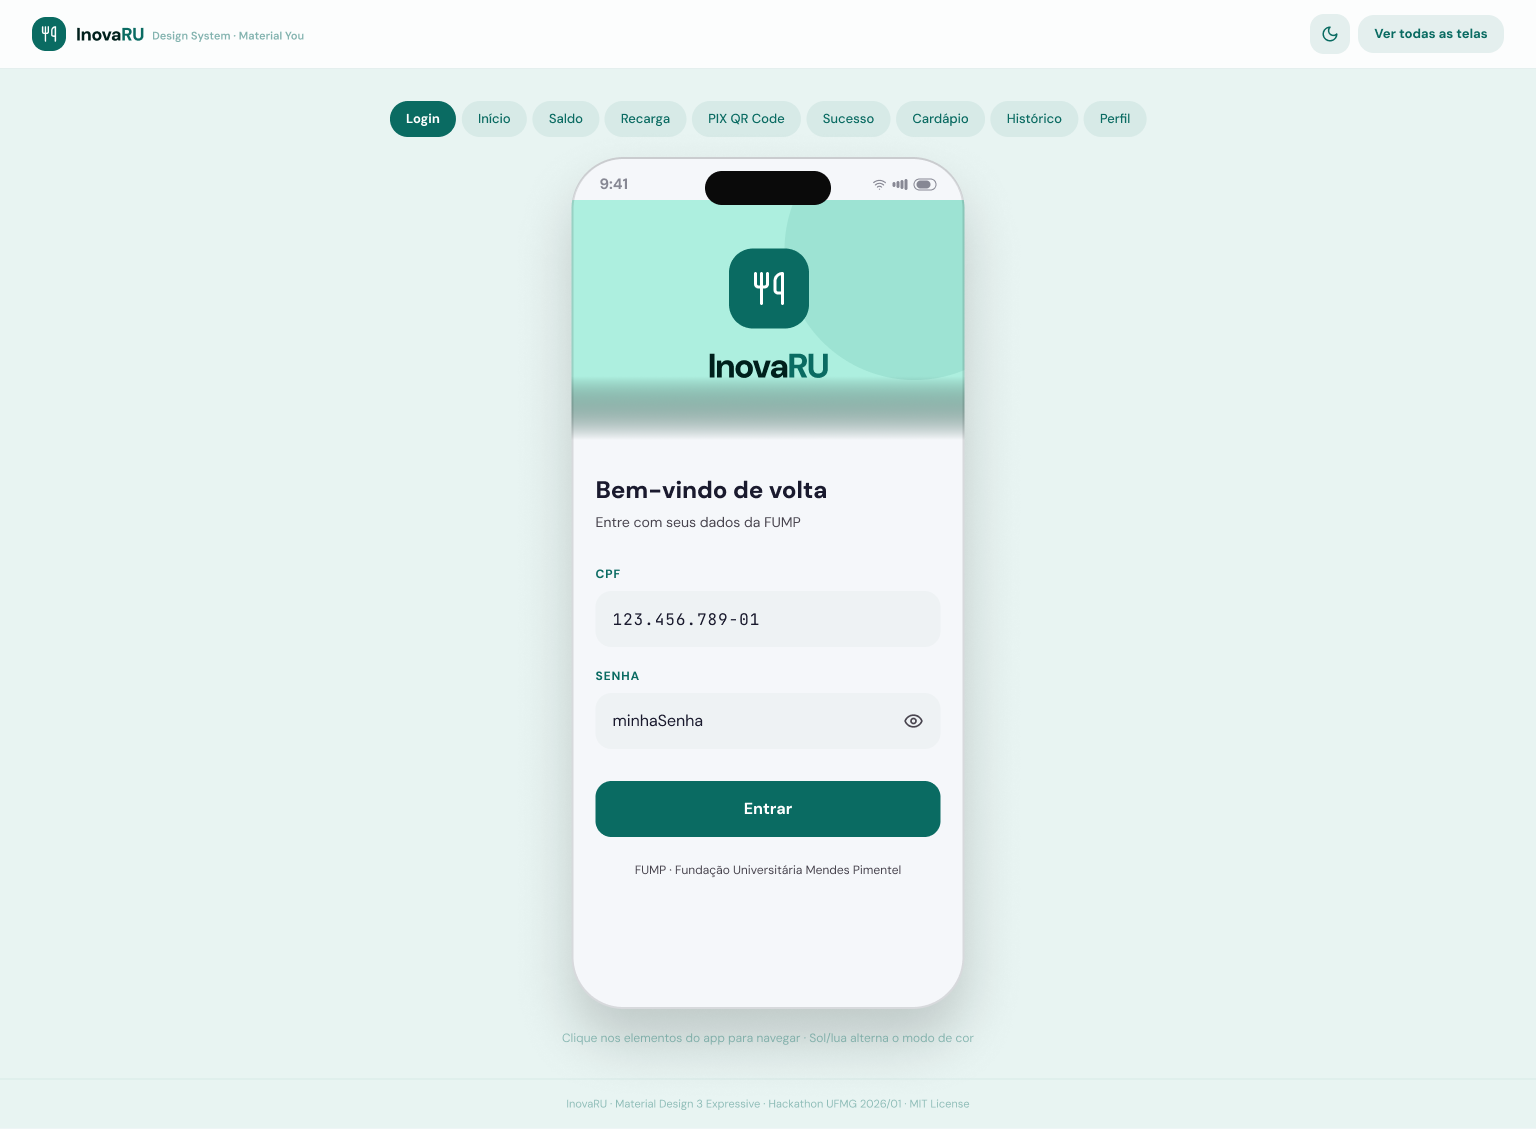
\includegraphics[width=\linewidth]{images/01-login.png}\\
            \captionof{figure}{Login}
        \end{column}
        \begin{column}{0.42\textwidth}
            \centering
            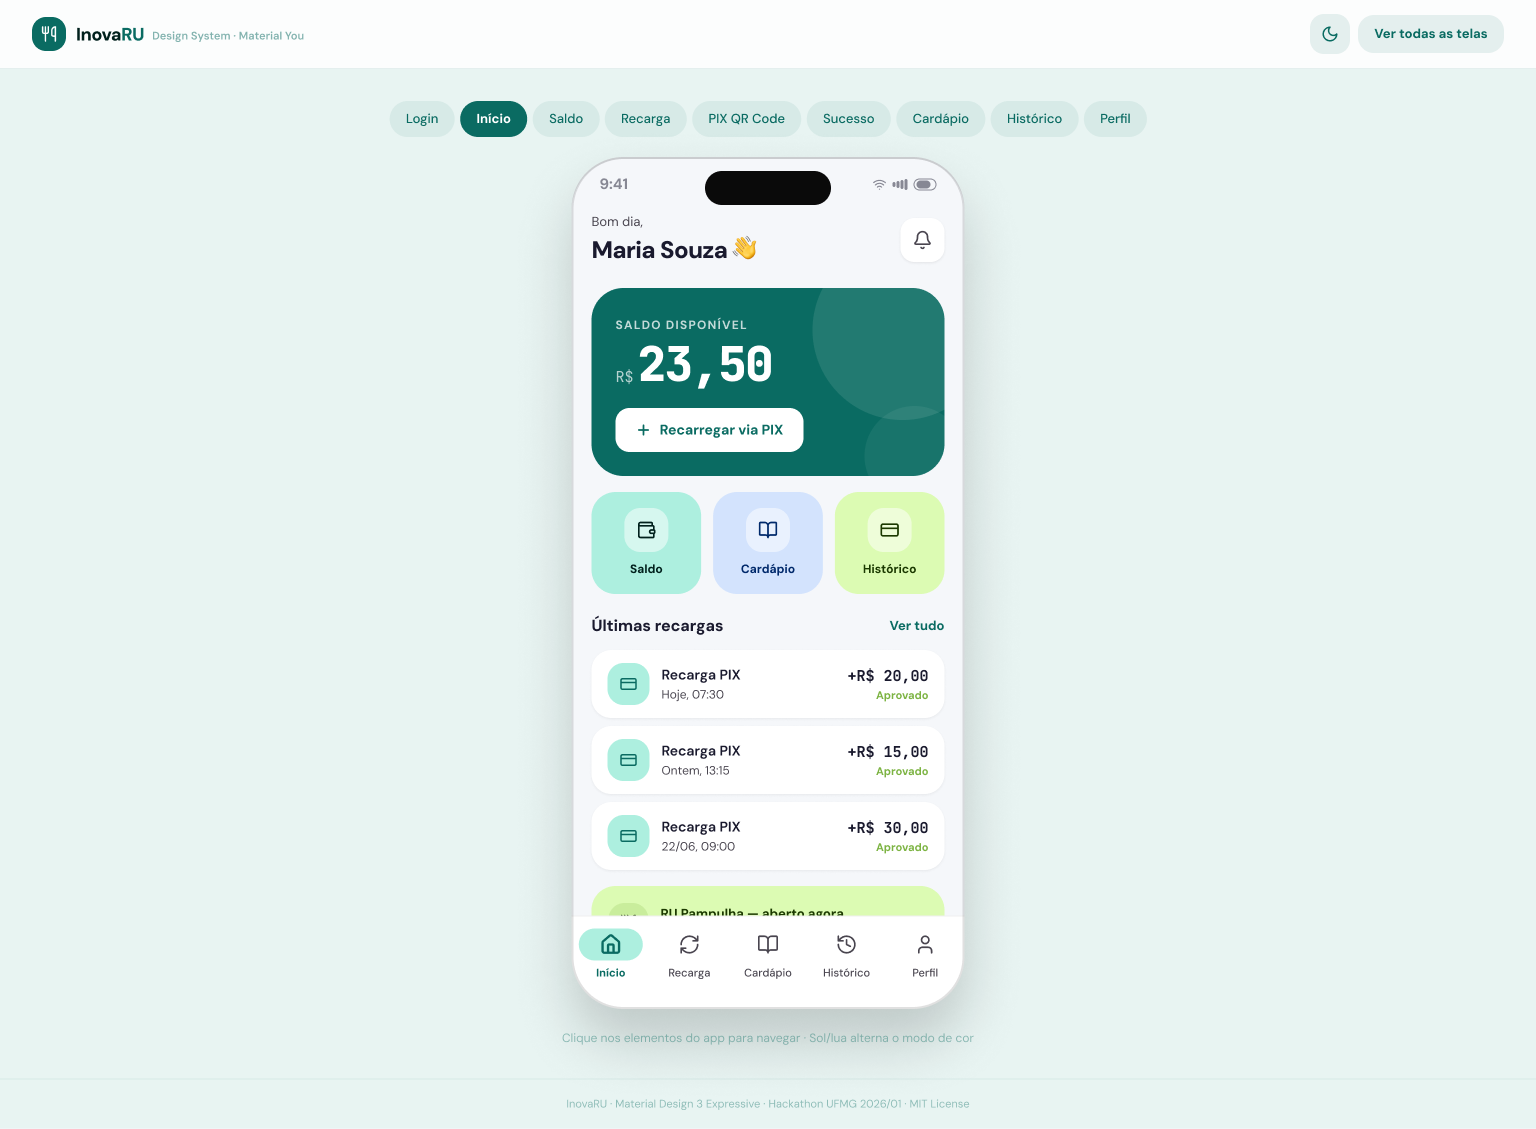
\includegraphics[width=\linewidth]{images/02-inicio.png}\\
            \captionof{figure}{Início}
        \end{column}
    \end{columns}
    \vspace{0.3cm}
    \begin{block}{Entrada sem fricção}
        \small
        Login com CPF (11 dígitos) + senha institucional da FUMP --- sem criar conta nova. Home com saudação, saldo em destaque e acesso rápido a Cardápio e Histórico.
    \end{block}
\end{frame}

\begin{frame}{Saldo e Recarga}
    \begin{columns}[T]
        \begin{column}{0.42\textwidth}
            \centering
            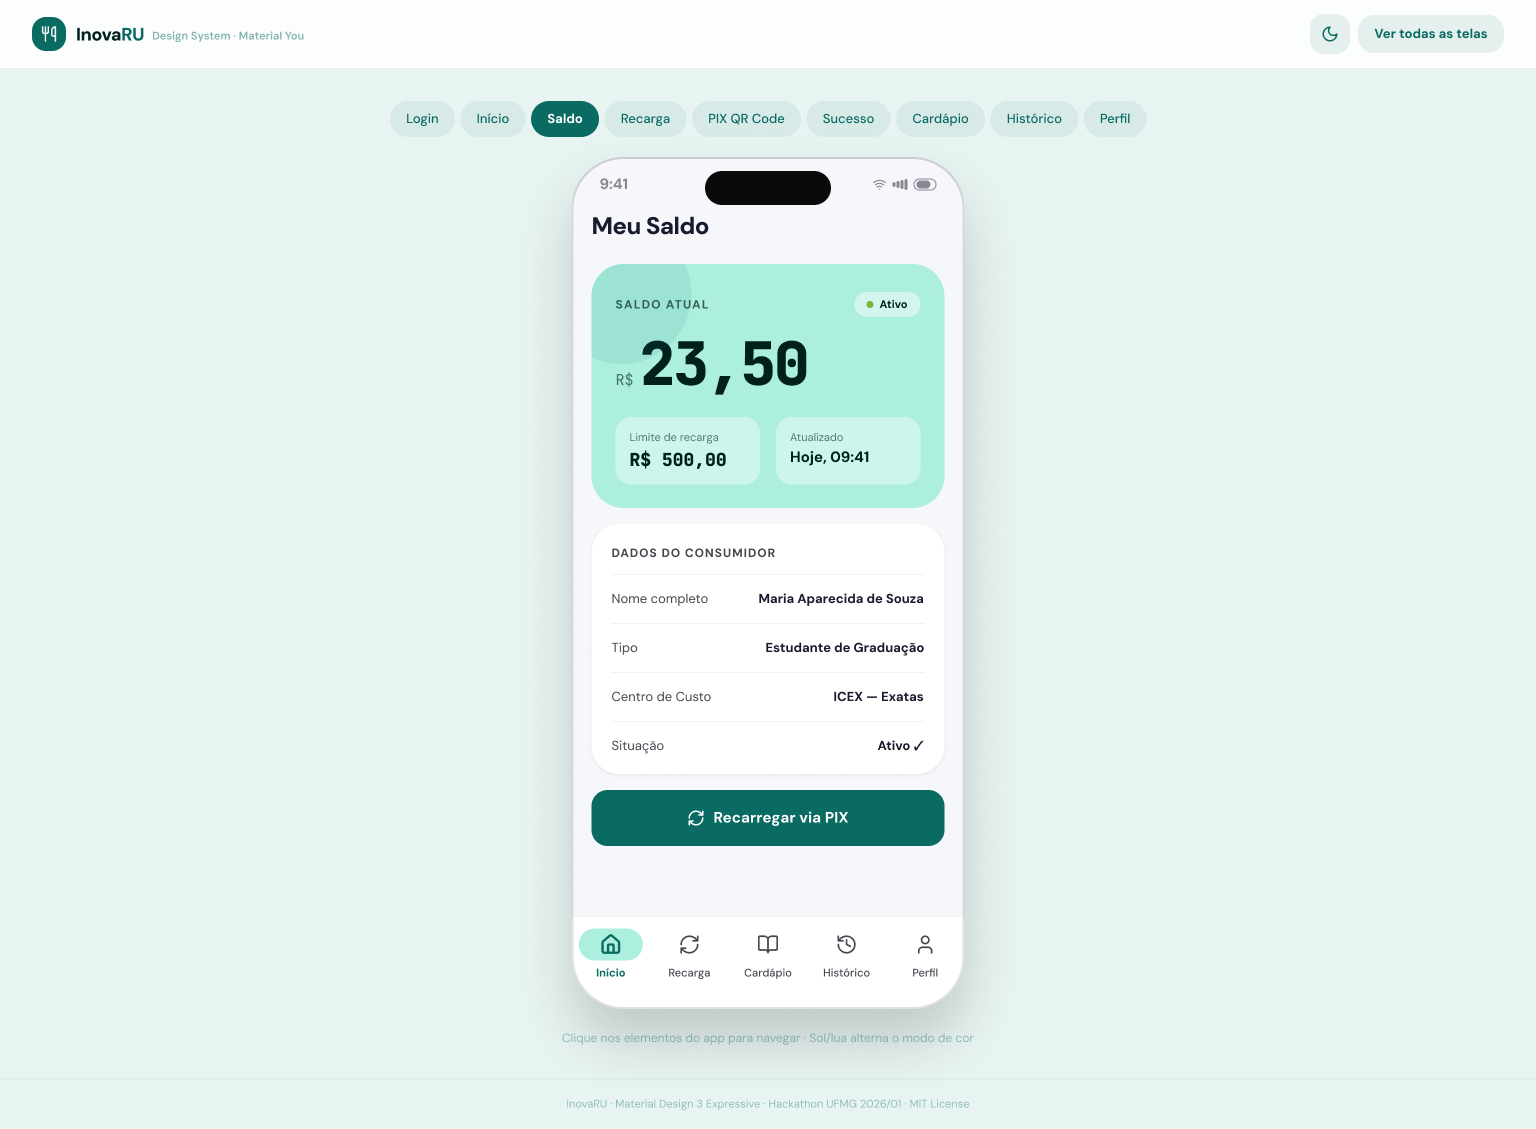
\includegraphics[width=\linewidth]{images/03-saldo.png}\\
            \captionof{figure}{Saldo}
        \end{column}
        \begin{column}{0.42\textwidth}
            \centering
            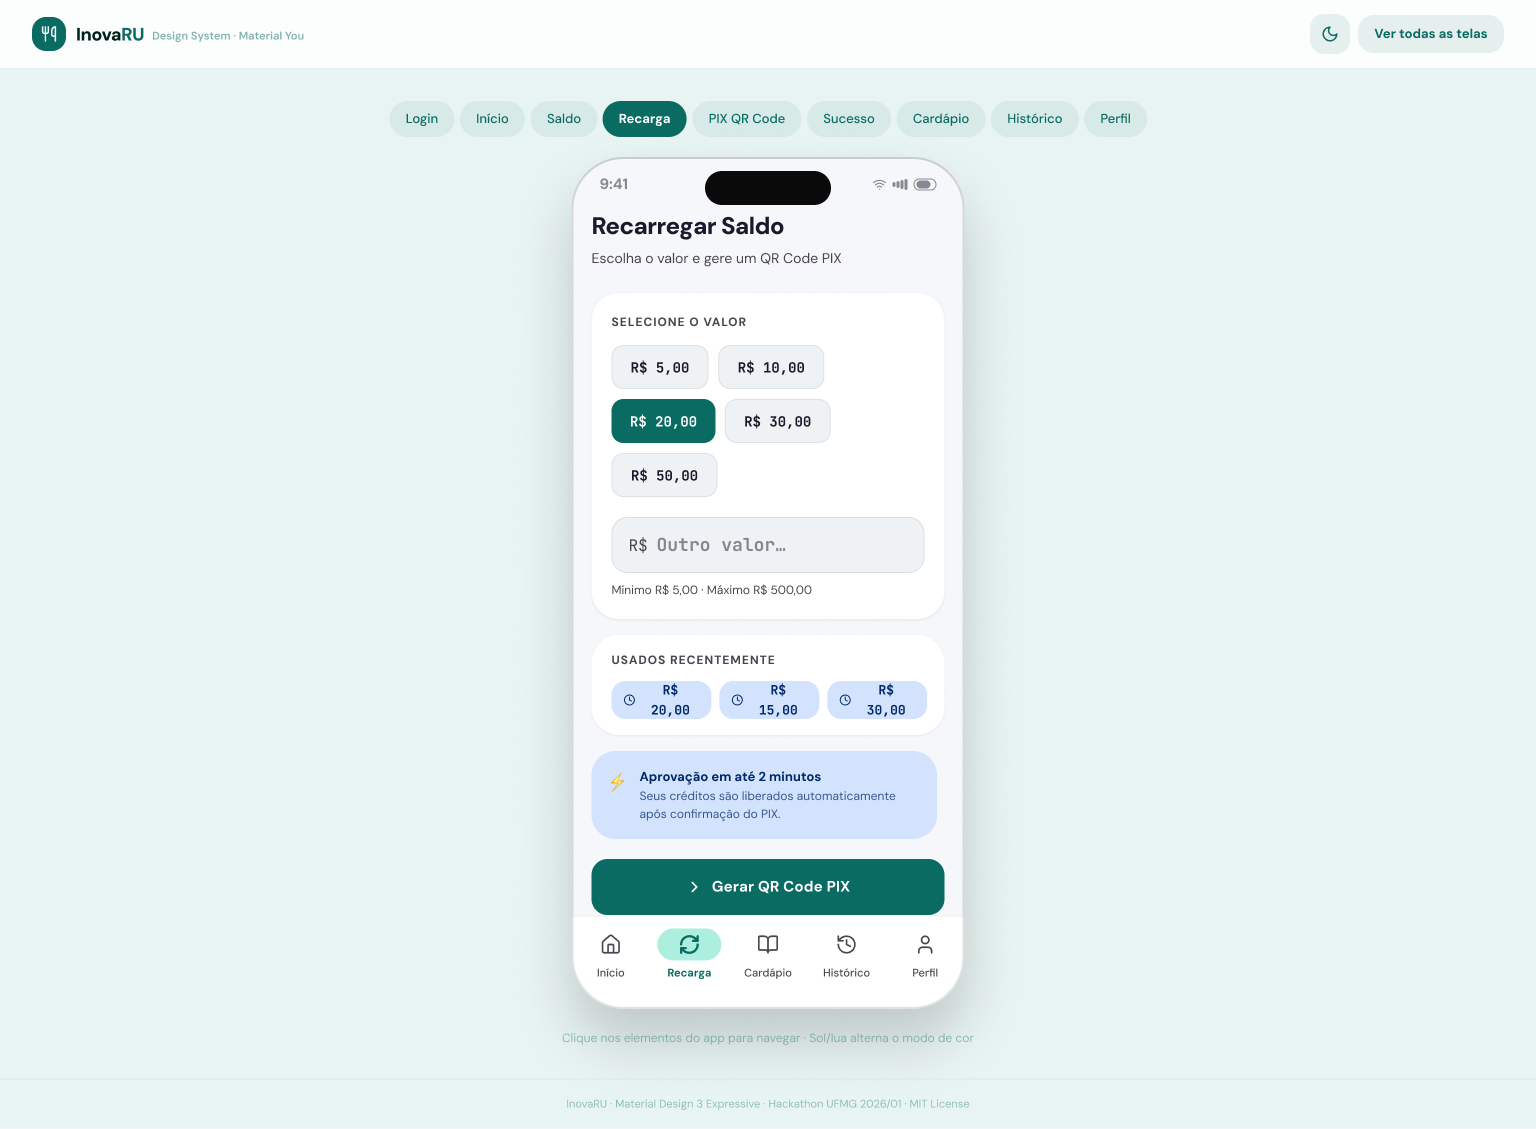
\includegraphics[width=\linewidth]{images/04-recarga.png}\\
            \captionof{figure}{Recarga}
        \end{column}
    \end{columns}
    \vspace{0.3cm}
    \begin{block}{Transparência e agilidade}
        \small
        Saldo detalhado, limite de recarga dinâmico e situação da conta. Na recarga: chips com os últimos valores usados + campo livre para digitar qualquer valor.
    \end{block}
\end{frame}

\begin{frame}{PIX e Confirmação}
    \begin{columns}[T]
        \begin{column}{0.42\textwidth}
            \centering
            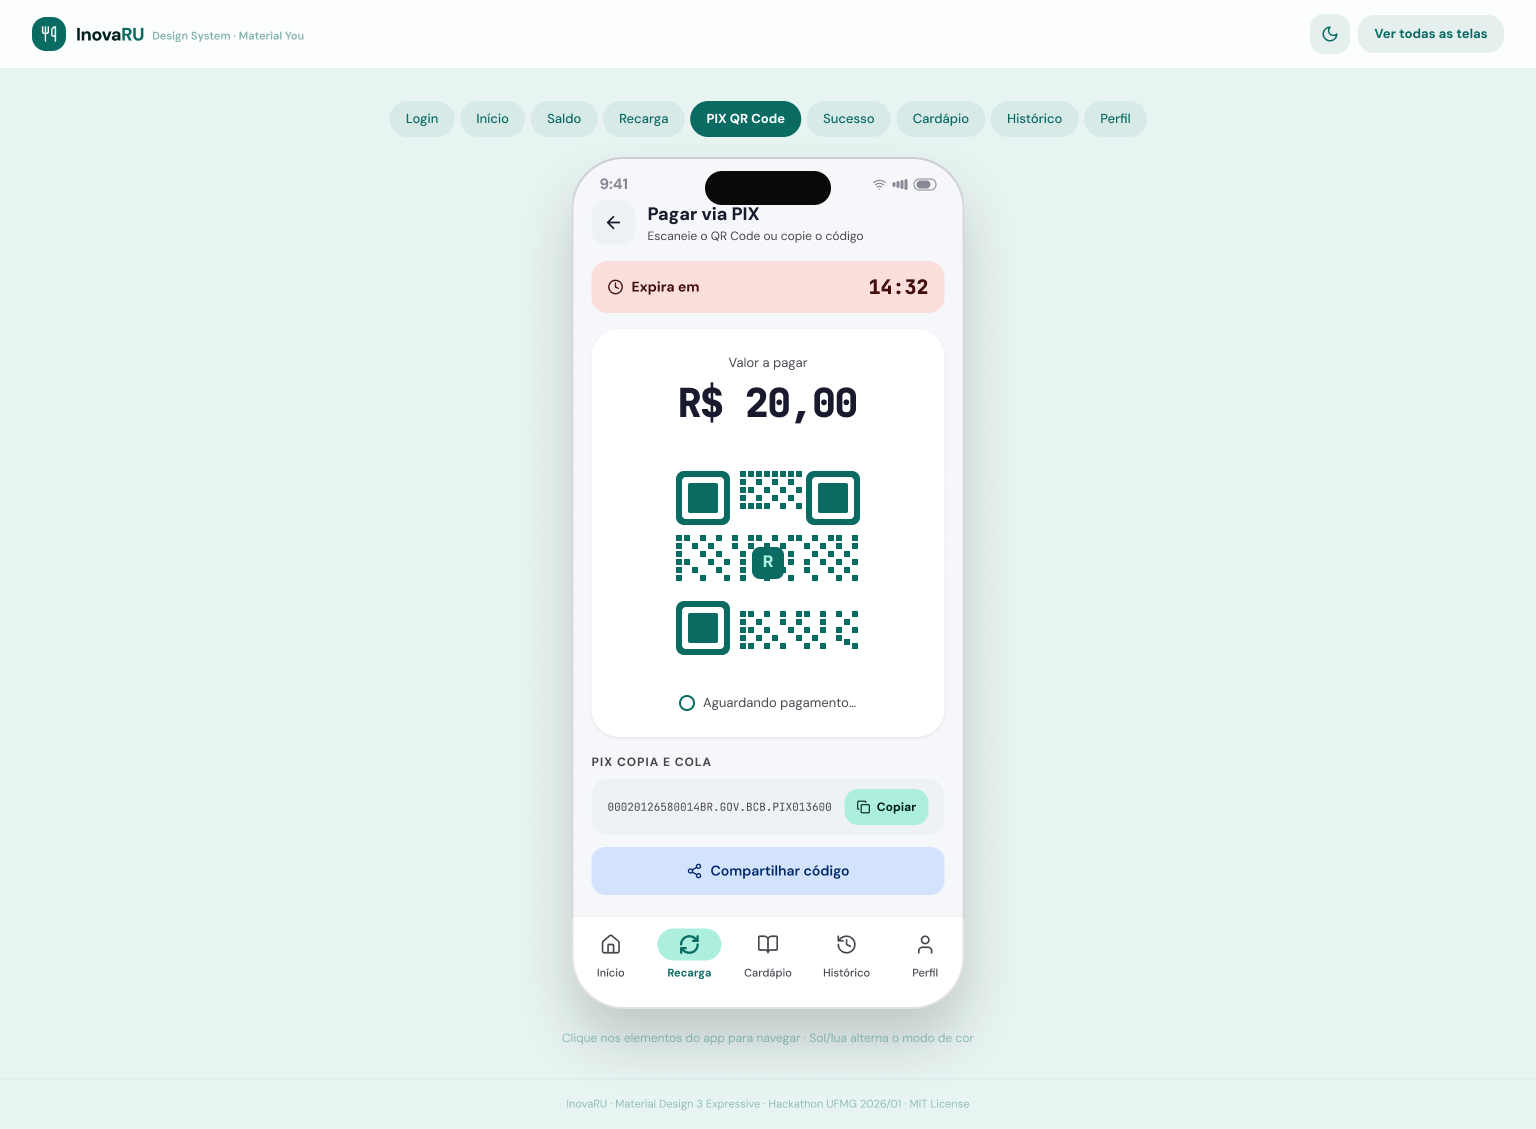
\includegraphics[width=\linewidth]{images/05-pix-qr-code.png}\\
            \captionof{figure}{QR Code PIX}
        \end{column}
        \begin{column}{0.42\textwidth}
            \centering
            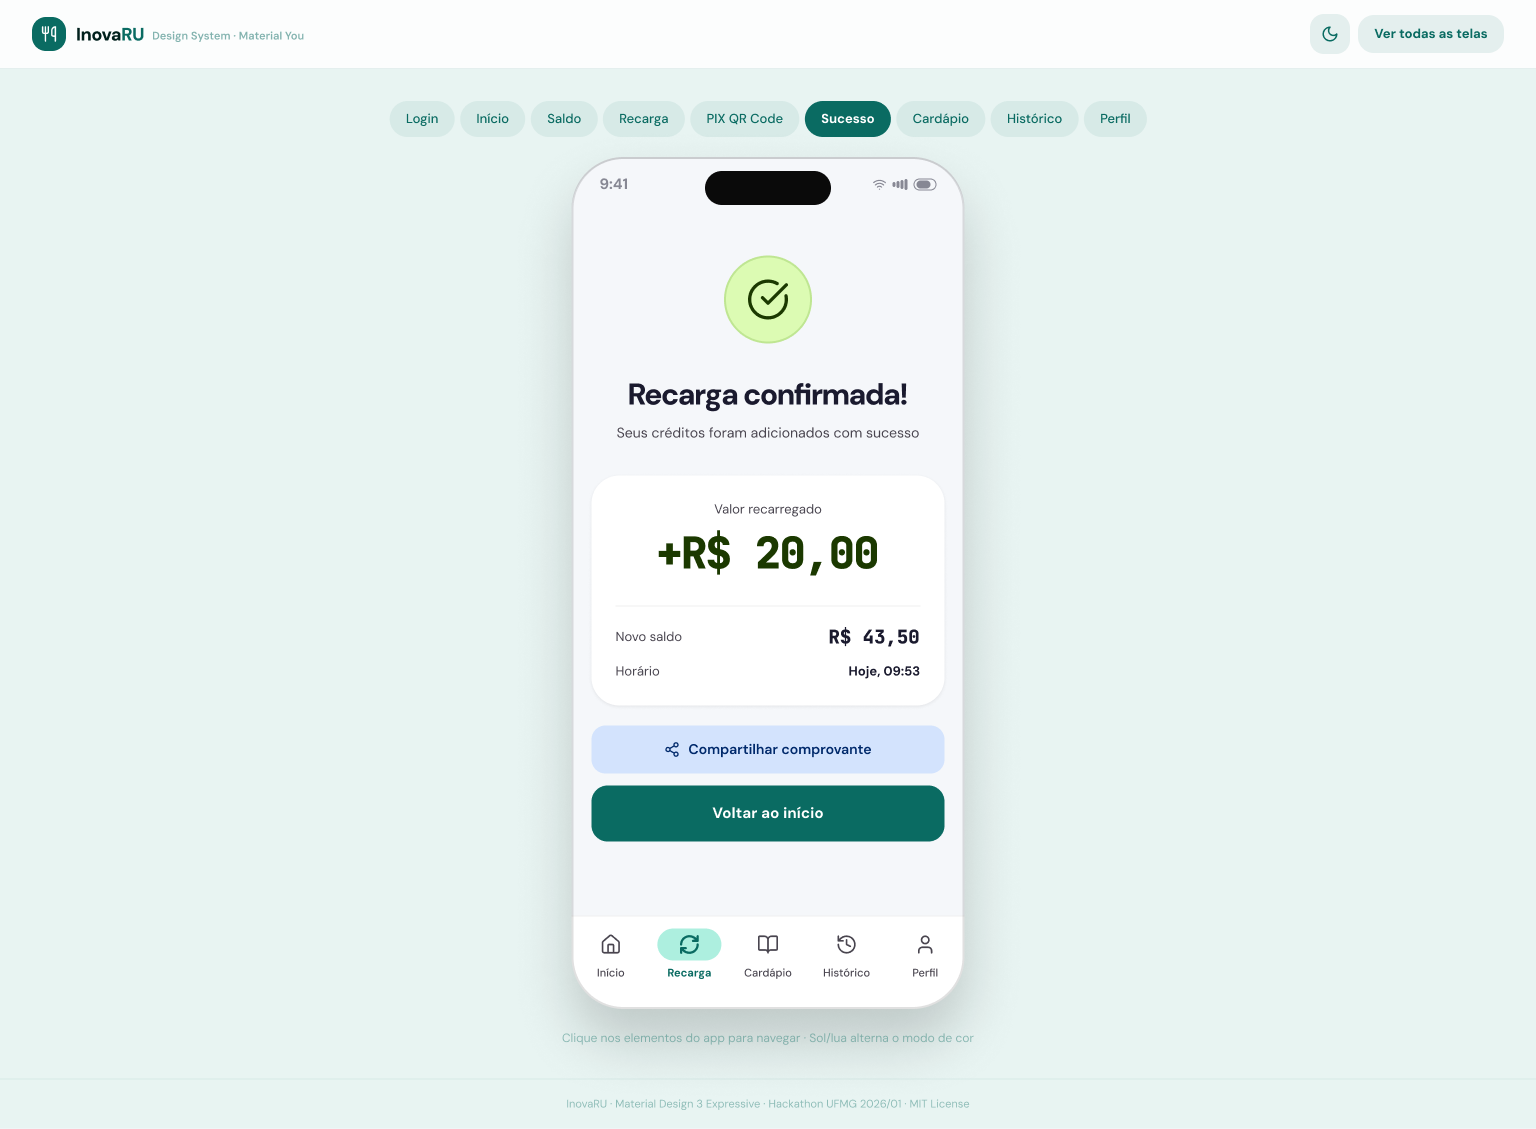
\includegraphics[width=\linewidth]{images/06-sucesso.png}\\
            \captionof{figure}{Sucesso}
        \end{column}
    \end{columns}
    \vspace{0.3cm}
    \begin{block}{Do QR ao saldo atualizado}
        \small
        QR Code e código copia-e-cola com contagem de expiração; confirmação automática por polling e tela de sucesso com o novo saldo, pronta para compartilhar.
    \end{block}
\end{frame}

\begin{frame}{Cardápio e Histórico}
    \begin{columns}[T]
        \begin{column}{0.42\textwidth}
            \centering
            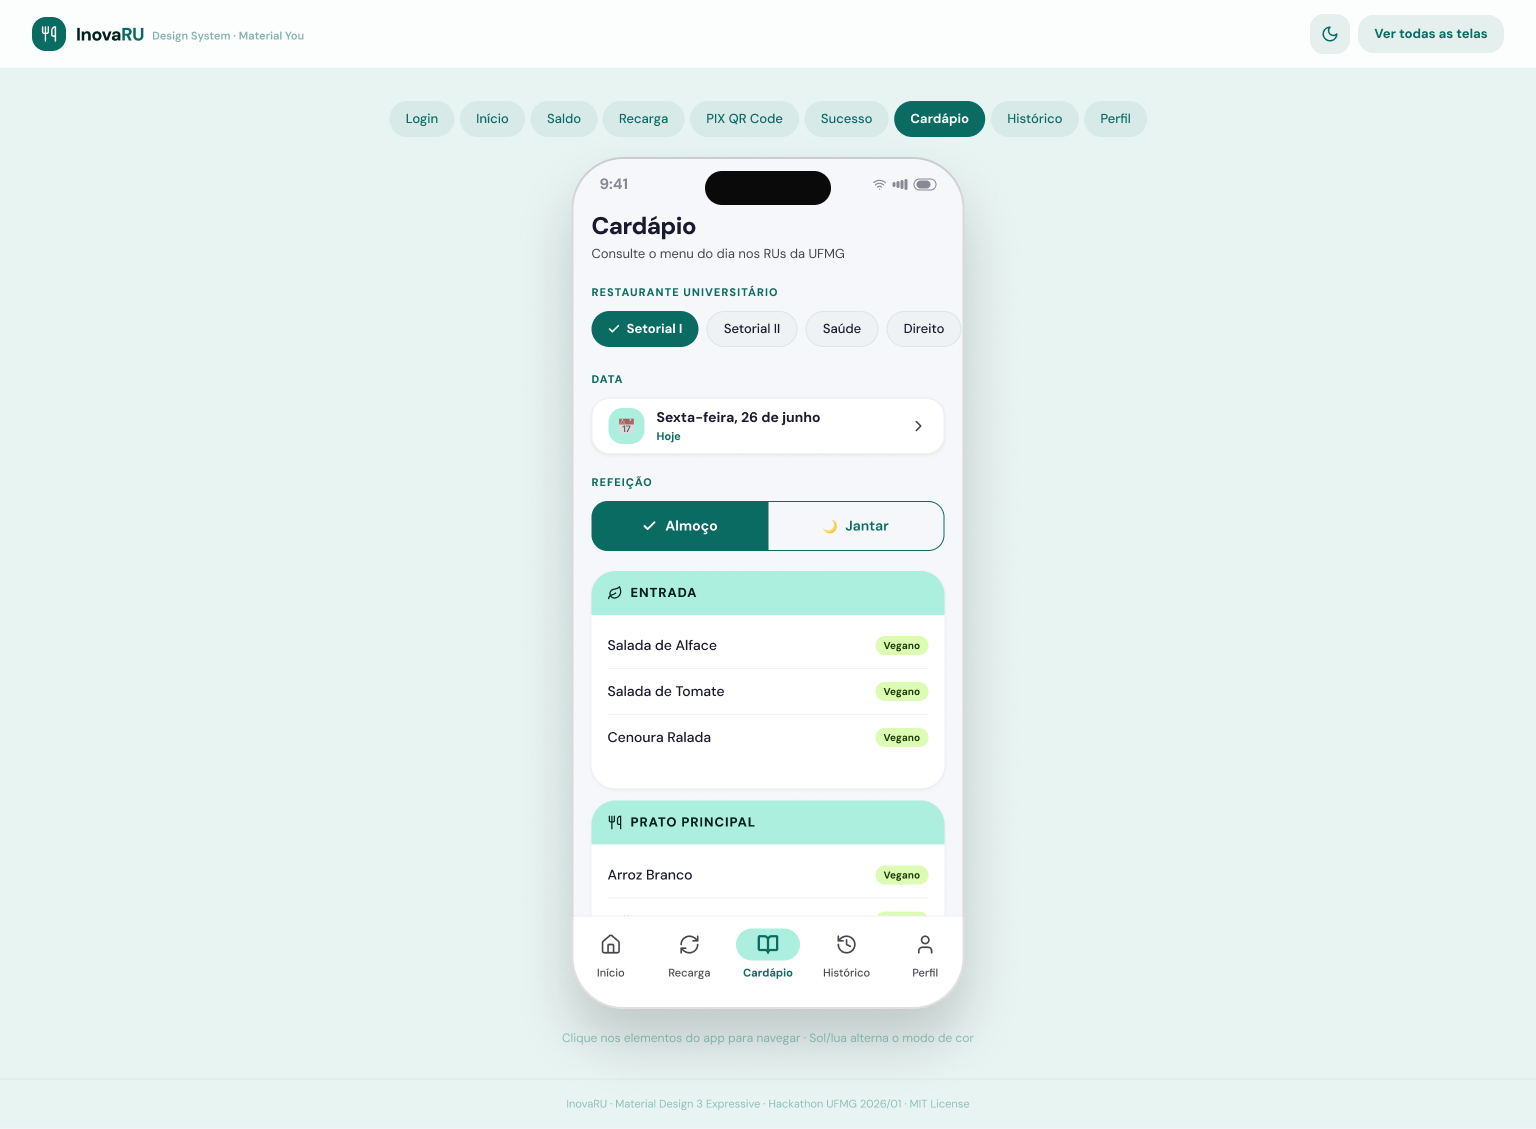
\includegraphics[width=\linewidth]{images/07-cardapio.png}\\
            \captionof{figure}{Cardápio do dia}
        \end{column}
        \begin{column}{0.42\textwidth}
            \centering
            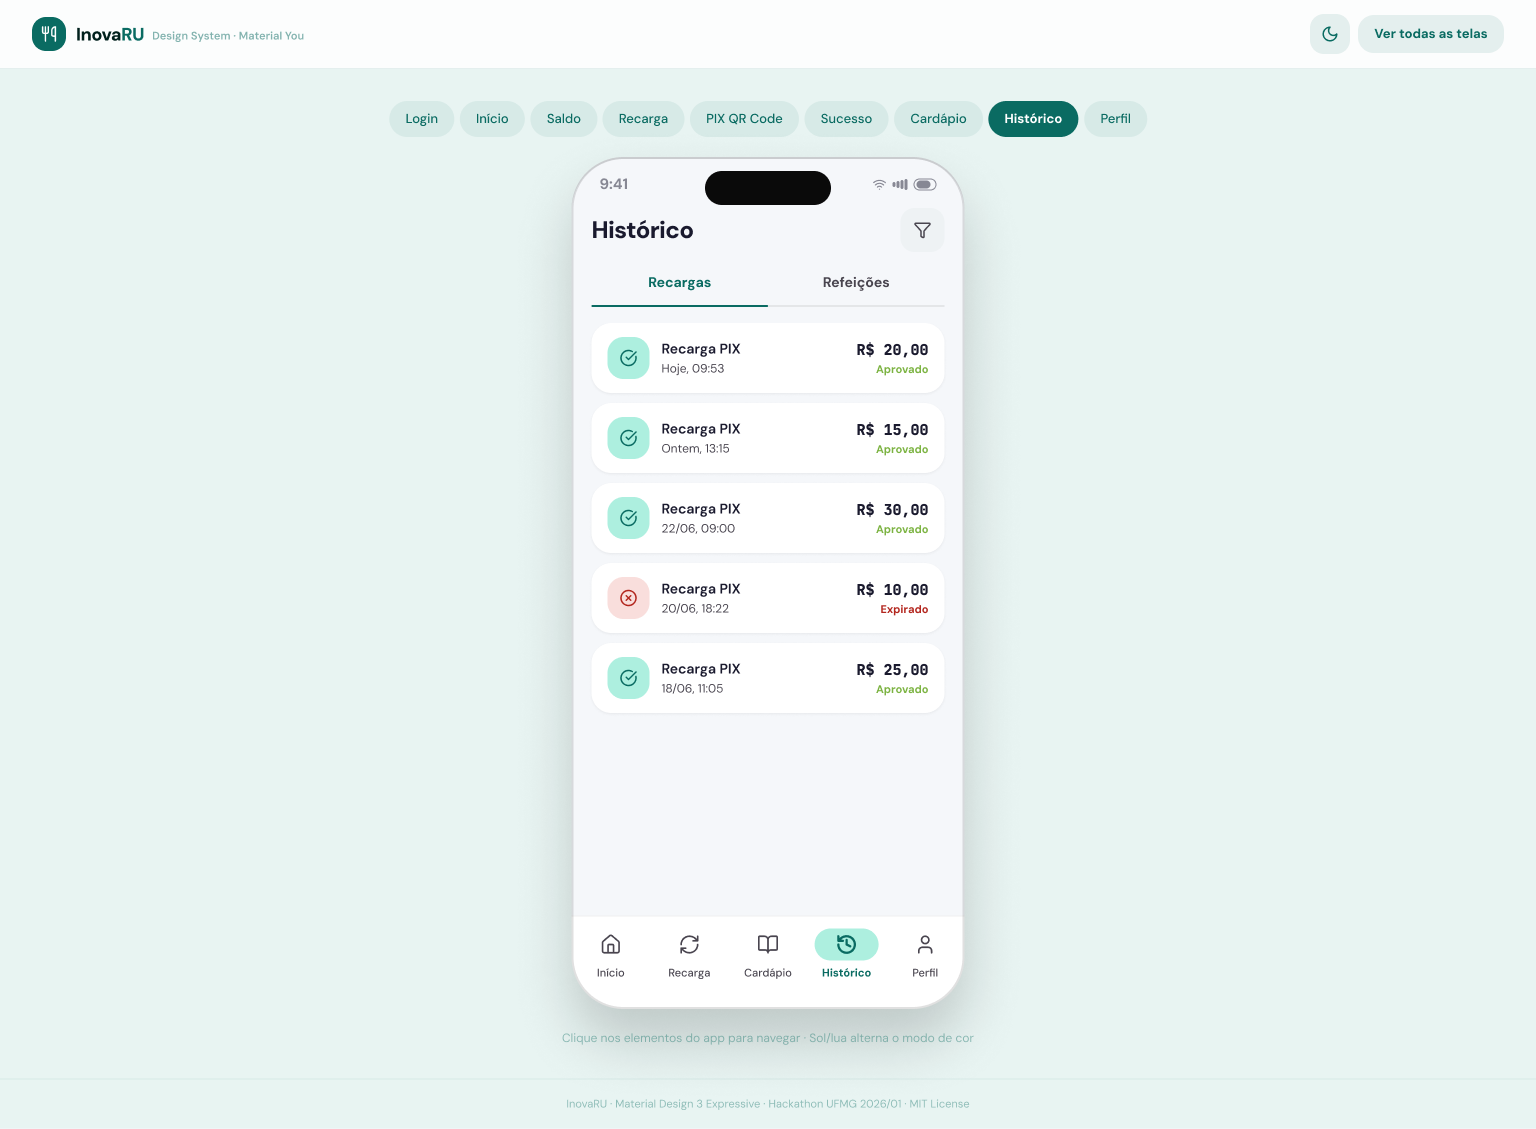
\includegraphics[width=\linewidth]{images/08-historico.png}\\
            \captionof{figure}{Histórico}
        \end{column}
    \end{columns}
    \vspace{0.3cm}
    \begin{block}{Rotina completa em um só app}
        \small
        Cardápio por RU com tags de restrição alimentar; histórico unificado de recargas e refeições, com filtro por data e RU, e paginação por scroll infinito.
    \end{block}
\end{frame}

\begin{frame}{Perfil}
    \begin{columns}[T]
        \begin{column}{0.5\textwidth}
            \centering
            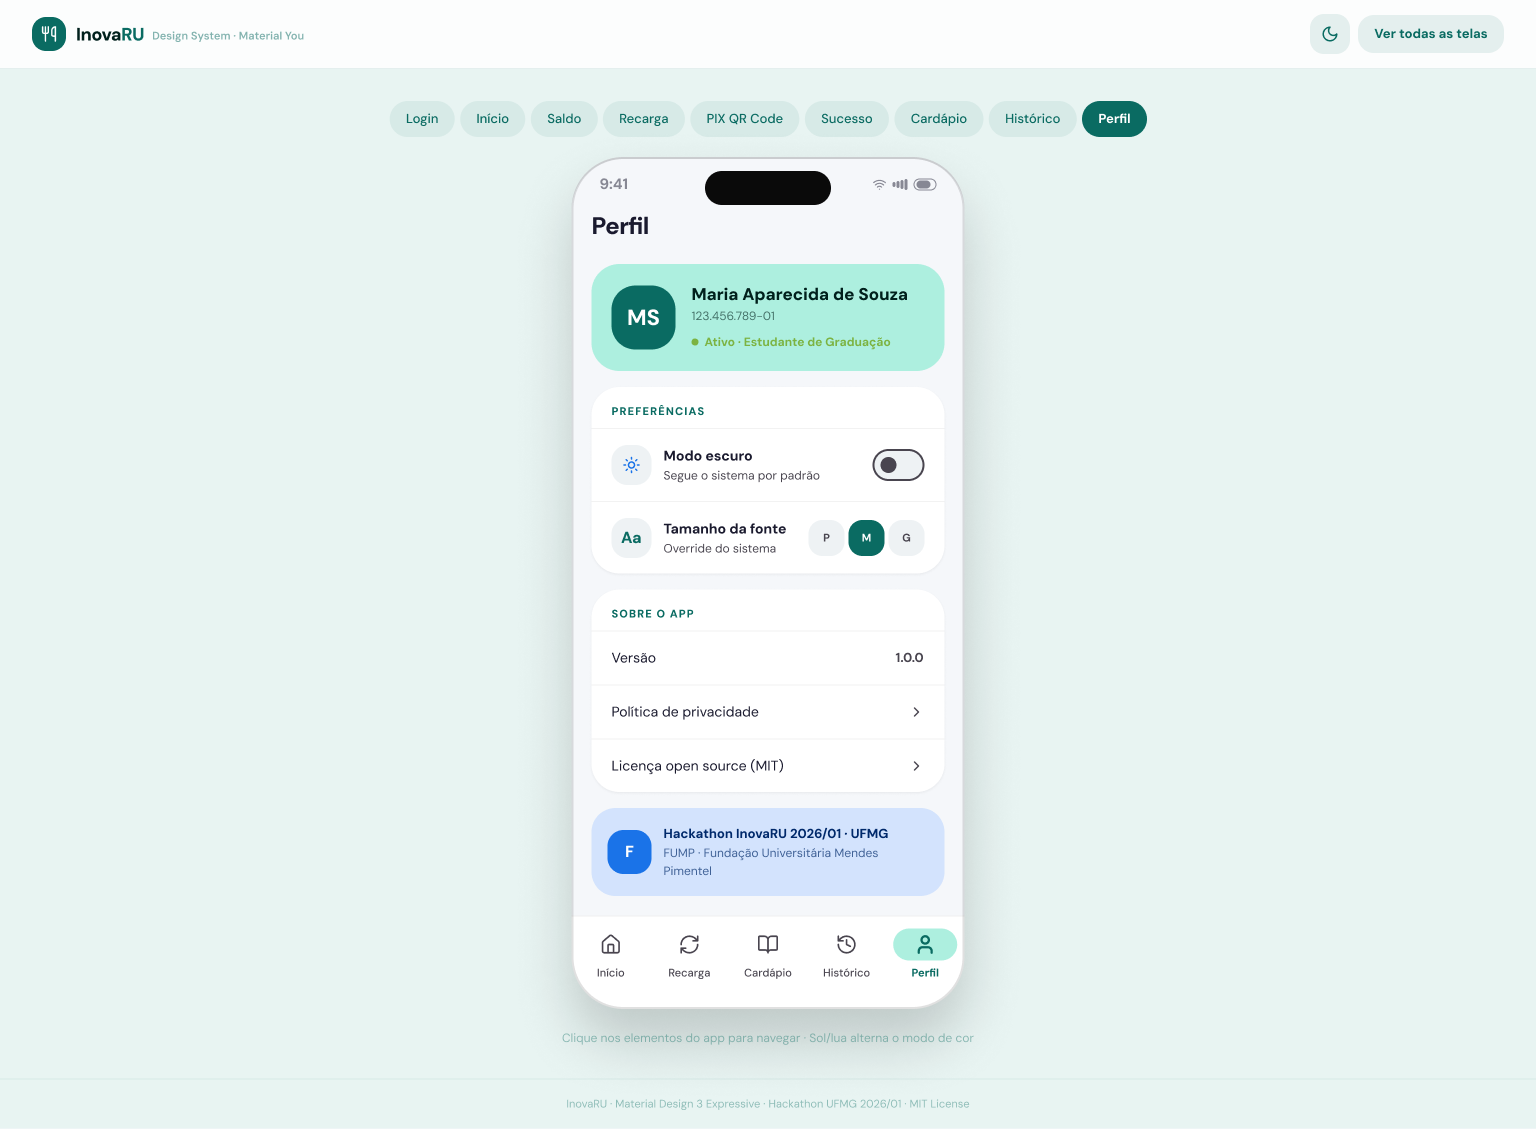
\includegraphics[width=0.85\linewidth]{images/09-perfil.png}\\
            \captionof{figure}{Perfil}
        \end{column}
        \begin{column}{0.42\textwidth}
            \begin{block}{Controle na mão do usuário}
                \small
                \begin{itemize}
                    \item Modo escuro: segue o sistema, com opção manual
                    \item Tamanho de fonte ajustável (P/M/G), além da escala do sistema
                    \item Dados da conta e situação (ativo/bloqueado)
                \end{itemize}
            \end{block}
        \end{column}
    \end{columns}
\end{frame}

\begin{frame}{Todas as Telas}
    \begin{center}
        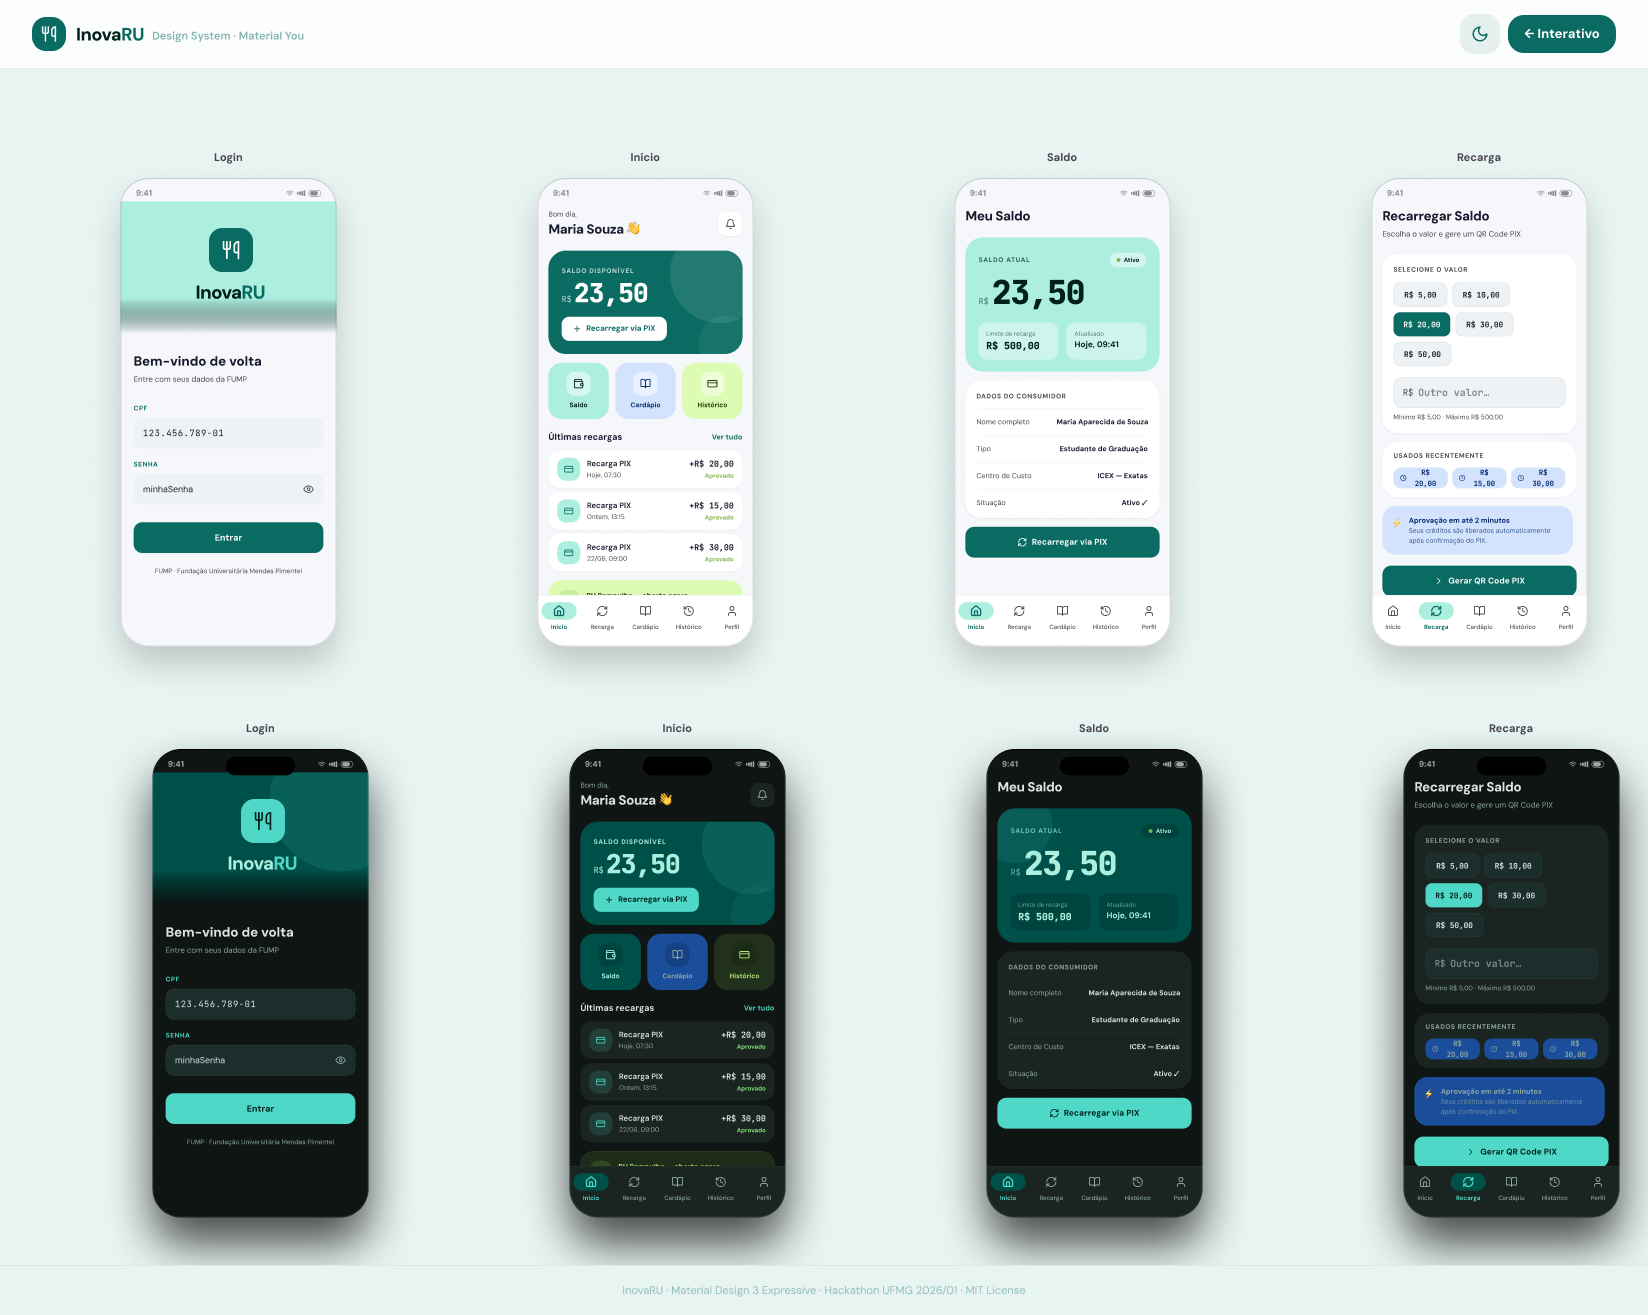
\includegraphics[height=0.72\textheight]{images/10-todas-telas.png}
    \end{center}
    \begin{center}
        \small\textit{Do login ao histórico, em modo claro e escuro --- consistente do início ao fim.}
    \end{center}
\end{frame}

% ============================================================
\section{Como Construímos}
% ============================================================

\begin{frame}{Stack Tecnológica e Segurança}
    \begin{columns}[T]
        \begin{column}{0.52\textwidth}
            \begin{block}{Stack}
                \small
                \begin{tabular}{@{}ll@{}}
                    \toprule
                    \textbf{Camada} & \textbf{Tecnologia} \\
                    \midrule
                    Mobile & React Native + Expo SDK 55 \\
                    Linguagem & TypeScript (strict) \\
                    Navegação & React Navigation v7 (tabs) \\
                    Estado servidor & TanStack Query \\
                    Estado cliente & Zustand \\
                    Estilo & NativeWind + Material You \\
                    Cache local & MMKV \\
                    Build & EAS Build (APK/AAB) \\
                    \bottomrule
                \end{tabular}
            \end{block}
        \end{column}
        \begin{column}{0.44\textwidth}
            \begin{alertblock}{Segurança em primeiro lugar}
                \small
                \begin{itemize}
                    \item JWT só em \texttt{expo-secure-store} (keystore nativo) --- nunca AsyncStorage
                    \item Senha nunca persistida no dispositivo
                    \item \texttt{X-Idempotency-Key} em toda criação de pagamento
                    \item HTTPS obrigatório; licença livre (MIT)
                \end{itemize}
            \end{alertblock}
        \end{column}
    \end{columns}
\end{frame}

\begin{frame}{Acessibilidade}
    \begin{columns}[T]
        \begin{column}{0.48\textwidth}
            \begin{block}{Para todo mundo usar}
                \small
                \begin{itemize}
                    \item Navegação completa por TalkBack (leitor de tela)
                    \item Switch Access funcional em todas as telas
                    \item Toques de no mínimo 48$\times$48dp
                    \item Fonte ajustável --- no sistema e dentro do app
                    \item Respeita a preferência de \textit{reduzir movimento}
                \end{itemize}
            \end{block}
        \end{column}
        \begin{column}{0.48\textwidth}
            \begin{exampleblock}{Além do mínimo do edital}
                \small
                \begin{itemize}
                    \item Contraste WCAG AA em todo o texto (4.5:1)
                    \item Contraste \textbf{WCAG AAA (7:1)} em saldo e valores de pagamento
                    \item Erro nunca indicado só por cor: sempre ícone + texto + cor
                    \item Títulos de seção com hierarquia semântica correta
                \end{itemize}
            \end{exampleblock}
        \end{column}
    \end{columns}
\end{frame}

\begin{frame}{Originalidade}
    \begin{block}{Não é só "mais um app de pagamento"}
        \small
        \begin{itemize}
            \item Ataca a \textbf{causa} da fila --- o gargalo de recarga --- em vez de só digitalizar o processo do caixa
            \item Une saldo, recarga PIX, cardápio e histórico em um único fluxo, sem apps separados
            \item Identidade visual \textbf{Material You dinâmica}: extrai cor do papel de parede do estudante (Android 12+), com paleta FUMP/UFMG como base
            \item Desenhado desde o início para baixa conectividade real de campus, não só para o cenário ideal
            \item Componentes e tokens pensados para futura integração no ecossistema de apps da FUMP
        \end{itemize}
    \end{block}
\end{frame}

% ============================================================
\section{Fechamento}
% ============================================================

\begin{frame}{Critérios de Avaliação e Equipe}
    \begin{columns}[T]
        \begin{column}{0.62\textwidth}
            \begin{block}{Edital, item 6.2}
                \scriptsize
                \begin{tabular}{@{}p{3.1cm}p{5.3cm}c@{}}
                    \toprule
                    \textbf{Critério} & \textbf{Onde entregamos} & \textbf{Peso} \\
                    \midrule
                    Usabilidade e Acessibilidade & MD3, WCAG AA/AAA, TalkBack, fluxo $<$30s & Alto \\
                    Originalidade & Ataque direto à fila + app unificado & Médio \\
                    Viabilidade e Integração & Fiel à especificação e aos endpoints FUMP & Alto \\
                    Código e Versionamento & Git contínuo, README, licença livre & Médio \\
                    \bottomrule
                \end{tabular}
            \end{block}
        \end{column}
        \begin{column}{0.34\textwidth}
            \begin{alertblock}{Equipe InovaRU}
                \small
                \begin{itemize}
                    \item Igor Martins
                    \item Ítalo Leal
                    \item Vítor Hugo
                \end{itemize}
            \end{alertblock}
        \end{column}
    \end{columns}
\end{frame}

\begin{frame}[standout]
    Obrigado!\\
    \Large Perguntas ou sugestões?
\end{frame}

\end{document}
